\chapter{CMS}

\section{Generelles}
Ein \textbf{Content-Management-System} (kurz CMS, deutsch Inhaltsverwaltungssystem) ist eine Software zur gemeinschaftlichen Erstellung, Bearbeitung und Organisation von Inhalten (Content) zumeist in Webseiten, aber auch in anderen Medienformen.
In einer \textbf{N-Tier Architektur} bildet ein oder mehreren Server einen Tier wobei jeder Tier eine wohldefinierte Rolle besitzt. Tiers sind über das Netzwerk miteinander verbunden.

\begin{figure}[h!]
\centering
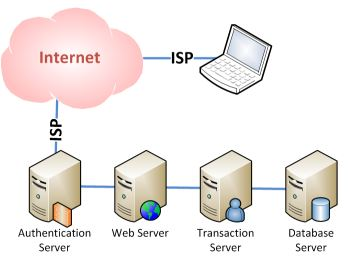
\includegraphics[width=0.7\linewidth]{fig/cms-generelle-referenz-architektur}
\caption{Generelle Referenz-Architektur}
\label{fig:cms-generelle-referenz-architektur}
\end{figure}

\emph{Die Abbildung \ref{fig:cms-generelle-referenz-architektur} soll zeigen, dass es eine oder mehrere Verbindung zum Internet durch verschiedene ISPs geben soll. Im Bild sind die vielen Netzwerkomponenten wie Router, Firewall, Switches nicht ersichtlich. Transaction Server und Applikation Server sind Synonme, beide wicklen Businesslogik ab.}

Als \textbf{Server} wird ein Prozess auf einem Host (Programm) aber auch ein Host in einem Netzwerk (Maschine) bezeichnet. Die erste Bezeichnung trifft es oft besser, denn es können verschieden Server auf einem und demselben Host laufen. Wobei die angebotene Funktionalität von der Art der Software, dem Netzwerkstack, dem BS sowie der Hardware abhängt.

In der \textbf{eBusiness Architektur} ist wichtig zu wissen, dass nicht nur der eigene Tier-Stack funktionieren muss, sondern übers Internet oft auch Third-party services angebunden werden (Ads, Payment usw.).

Ein \textbf{Web-Server} handhabt das HTTP Protokoll. Einzelne Connections bei HTTP 1.0 und persistente Connections bei HTTP 1.1 und nun kommt HTTP 2.0 (SPDY). Web-Server laufen in Multi-Process oder Multi-Threaded Modus. Der Multi-Threaded Modus ist sexier, aber kann den ganzen Prozess in Mitleidenschaft ziehen, falls was schief geht. Multi-Prozess ist teurer aber arbeiten vollständig unabhängig.

Vielfach wird die Prüfung der Identität durch den Web Server durchgeführt, welche somit auch die Rolle des \textbf{Authentisierungs Server} einnimmt.

Der \textbf{Applikation Server} ist zuständig für die dynamische Seitenerzeugung. Beinhaltet die Business-Logik. Beinhaltet die Session-Steuerung. Es können Standalone Applikationen, welche vom App Server ausgeführt werden (CGI, Fast CGI) oder Server-side Scripting, welche durch den App-Server interpretiert werden (ASP, PHP oder JSP).

Ein \textbf{Datenbank Server} speichert für die Applikation notwendigen Daten. Komplexe Queries lassen sich als 'stored procedures' intern speichern, diese sind pre-compiliert und parametrisiert. Einen Datebank-Server zu optimieren bzw. zu skalieren ist oft schwierig (siehe Kapitel Skalierung).

CGI bedeutet \textbf{Common Gateway Interface} und stellt eine Standard-Schnittstellen zu externer Applikationssoftware dar. Bei CGI ist jeder Request ein neuer Prozess und bei Fast-CGI wird Multi-Threading verwendet.

\textbf{Sichere Kommunikation} mit dem Web Server kann über SSL/TLS verfolgen. Dabei nimmt aber die Serverperformance ab. Damit der Server HTTPS nutzt, muss der Admin ein Public-Zertifikat erzeugen (CSR). Dieses muss durch eine CA (certifcate authority) signiert werden. Die Idendität des Web Servers wird damit bestätigt. 

\begin{figure}[h!]
	\centering
	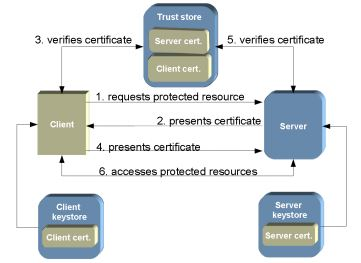
\includegraphics[width=0.7\linewidth]{fig/cms-ablauf-verifikation-von-zertifikaten}
	\caption{Verifikation von Zertifikaten}
	\label{fig:cms-ablauf-verifikation-von-zertifikaten}
\end{figure}

\subsection{Sessions}
Die Zustandslosigkeit des HTTP Protokoll führt dazu, dass Entwickler den Status auf Stufe Applikation implementieren muss - was in \textbf{Sessions} mündet. Damit die beliebten Warenkorbs in den Webshops realisiert werden können, gibt es verschiedene Möglichkeiten:
\begin{description}
	\item[URL rewriting:] Alle Links auf einer Seite bei der Auslieferung modifizieren und mit einem Session Key bestücken. Falls der Link herumgereicht wird, kann die Session übernommen werden.
	\item[Verstecke form-Variabeln:] Man versteckt den Session Key in der Form Variabeln. Ist immerhin sicherere als die obere Variante, aber ist natürlich absoluter Müll, da nun immer POST-Requests gemacht werden müssen. Die Navigation ist Form-based keine typischen Links <a> möglich.
	\item[Cookies:] Session Key in einem kleinen Informationsspeicher - dem Cookie - ablegen. Ein Cookie ist ein 4-Tuple aus Name, Werte, Ablaufdatum, Domain. Achtung: Nur kleine Datenmengen, Cookies können manipuliert werden, Client kann Cookies verweigern.
\end{description}

\subsection{Netzwerk Infrastruktur}

\begin{figure}[h!]
	\centering
	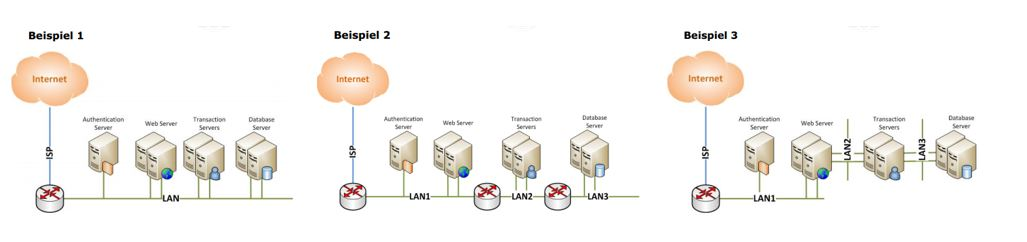
\includegraphics[width=1\linewidth]{fig/cms-netzwerkinfrastruktur}
	\caption{Netzwerk Infrastruktur}
	\label{fig:cms-netzwerkinfrastruktur}
\end{figure}

Beispiel 1: Zeigt, dass alle Server hinter dem Router im selben Netz sind. Umso mehr Elemente im gleichen Netz sind umso mehr wird das Netzwerk belastet und warum sollte der Web Server im gleichen Netz wie der DB Server sein? Diese dürfen sowieso nicht miteinander schwatzen.

Beispiel 2: Für jeden Tier sein eigens Netz. Nun haben wir etwas mehr Sicherheit, aber Routing ist teuer! Um an den DB Server zu gelangen muss nun immer über 3 Router gegangen werden.

Beispiel 3: Jeder Tier befindet sich in zwei Netzen. Dies erfordert einfach, dass jeder Server zwei NICs hat. Hier wird dafür Switching verwendet, welches performanter als Routing ist.

\textbf{Internet-Verbindungen} sollten redundant ausgelegt werden. Die minimale Bandbreite muss garantiert werden und übliche Bandbreiten sind >= 100 MBit/S.

\subsection{Performance-Indikatoren}
\begin{description}
	\item[Latenz (Latency):] Benötigte Zeit um eine 0 Byte grosse Seite auszuliefern. Einheit: http/s oder s/http
	\item[Durchsatz (Throughput):] Maximale Geschwindigkeit mit der eine (unendlich grosse) Seite gesendet werden kann. Einheit: Bytes/s oder Mbytes/s.
	\item[Requests:] Wie viele Requests pro Sekunden gemacht werden können. Einheit: Anzahl Request/s.
	\item[Delay T:] T = Latency + ByteHTML / Throughput. Diese Gleichung gilt wenn die anderen Architekturelemente nicht üebrlastet sind und der Web-Server nicht seinen maximalen Workload erreicht hat. Beispiel: T= 0,1s + ((100KBytes) / (800KBytes/s)) = 0,225s
\end{description}

\section{Proxy}
Ein \textbf{Proxy} ist ein Stellvertreter oder auch Vermittler. Wir unterscheiden zwei Proxy-Arten:

\begin{description}
	\item[Forward Proxy:] Versteckt die Identität des Client vor dem Server. Der Client ruft einen Server über einen Proxy auf, dabei weiss der Server nicht, wer der konkrete Client ist.
	\item[Reverse Proxy:] Versteckt die Identität des Servers vor dem Client.  Dieser nimmt die Anfragen im Internet entgegen und leitet diese an andere Server im internen Netzwerk weiter. Der Anfragende verbindet sich nur mit dem Proxy, das interne Netzwerk muss nicht bekannt sein.
\end{description}

\begin{figure}[h!]
	\centering
	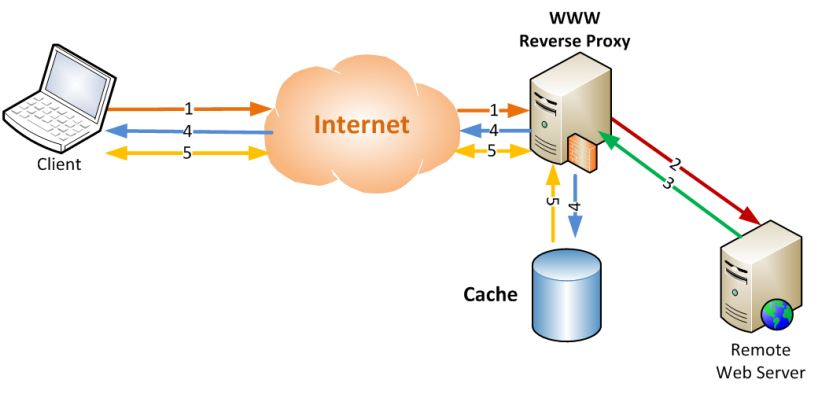
\includegraphics[width=0.7\linewidth]{fig/cms-reverse-proxy-cache}
	\caption{Reverse Proxy und Cache in Action}
	\label{fig:cms-reverse-proxy-cache}
\end{figure}

Oft wird die Funktionalität des Proxy sowie die des \textbf{Cache} in einem Server/Device angeboten. Der Cache speichert die Antwort des Client-Requests. Damit wird bei einem späteren Request eines Clients der Zugriff auf die Ressource ins Internet vermieden.

\section{Web Application Firewall}
Eine Web Application Firewall (WAF) werden oft auch \emph{Deep Packet Inspection Firewall} genannt und geht im Grundsatz auf zwei Fragen ein: Wer jemand ist und was er tut. WAFs suchen gezielt nach Signaturen einer Attacke oder nach abnormalen Verhalten. WAFs können als Reverse Proxy auf dem Weg zum Webserver installiert werden. Ein wesentlicher Vorteil ist, dass man bestehende Web-Applikationen \textbf{nachträglich absichern} kann, falls diese \textbf{keinen ausreichenden Schutz} gewähren. So muss man die Web-Applikation nicht umprogrammieren. Airlock ist eine sehr gute WAF, welche auch Load Balancing und Reverse Proxy kann. Gemäss Infanger sogar die beste und ein Produkt aus der Schweiz. Auf dem Markt existieren nur 5 WAFs, welche brauchbar sind.

\section{Load Balancer}
Leitet die Anfrage an einen 'freien' Server weiter und muss dafür kontinuierlich die Serverlasten messen. Das führt dazu, dass der Load Balancer Request-Queues verwalten muss. Dies wird oft mit einem Reverse Proxy oder WAF kombiniert. Hardware Load Balancer sind schneller dafür sind Software Load Balancer besser anpassbar. 

\subsection{DNS Round Robin}
Ein simple Idee wäre, dass gleich der DNS-Dienst eine Lastverteilung durchführt. Wenn ein Client X kommt, dann bekommt er die IP des Server A, wenn Client Y kommt dann bekommt er die IP des Server B. Aber das geht nur bedingt, da im DNS Bereich viel gecacht wird und nicht für jeden Request der DNS angefragt wird. Grosse Firmen benutzen dies schon auch. Ich denke, dass es beispielsweise Sinn machen kann, dass Netflix bei Anfragen aus Europa, dann die europäischen Netflix-Server zurückliefert und Anfragen in Amerika die entsprechenden Server dort.

\subsection{DNS und Reverse Proxy}
Über den DNS wird die IP des Reverse Proxy mitgeteilt. Das Load Balancing wird anschliessend vom Reverse Proxy vollständig umgesetzt.

\section{Skalierung}
Mit viralem Marketing kann in Sekundenschnelle sehr grossen Erfolg erzielt werden und dann möchte man von einem Moment auf den anderen Millionen von Benutzer bedienen ohne Downtime! Es gibt dazu mehrere \textbf{Variabeln}, welche wir bei der Skalierung berücksichtigen müssen:

\begin{description}
	\item[Scalability:] Die Anzahl von Benutzern / Sessions / Transaktionen / Operationen soll nicht beschränkt und beliebig erweiterbar sein. (möglichst hoch)
	\item[Performance:] Die Ressourcen sollen optimal genutzt werden. (hoch)
	\item[Responsiveness:] Dies bezieht sich auf die Zeit pro Operation. (hoch)
	\item[Availability:] Die Verfügbarkeit der Applikation. (hoch)
	\item[Downtime impact:] Auswirkung der Downtime auf beispielsweise die Anzahl Benutzer. (niedrig)
	\item[Kosten:] Natürlich soll alles nichts Kosten. (niedrig)
	\item[Maintenance Effort:] Wie viel Wartungsaufwand mit der Architektur verbunden ist. (niedrig)
\end{description}

Folgende \textbf{Faktoren} haben Einfluss auf Skalierungs-Möglichkeiten:
\begin{itemize}
	\item Platform selection
	\item Hardware
	\item Application Design
	\item Database/Datastore Structure and Architecture
	\item Deployment Architecture
	\item Storage Architecture
	\item Abuse prevention
	\item Monitoring mechanisms
\end{itemize}

\subsection{Skalierungs-Arten}
\begin{description}
	\item[Vertikal skalieren:] \emph{Scaling Up} - Wir können immer schnell vertikal skalieren. Man skaliert den einzelnen Node, einfach mehr Hardware reinbuttern. Aber irgendwann ist fertig. Hardware skaliert nicht linear. Benötigt Downtime und erhöht auch den Downtime Impact. Lineare Kosten wachsen exponentiell.
	
	\item[Vertikal partitionieren] Mit vertikaler Partitionierung lagern wir einzelne Tasks auf einzelne Server aus. Jeder Node ist somit anders als der andere. Dies kann auch auf unterschiedlichen Levels angegangen werden: Applikation, Server, Data, Hardware.
	Beispielsweise haben wir einen einzigen Server auf dem ein Web- sowie DB-Server läuft. Nun partitionieren wir vertikal und somit trennen wir Web- sowie DB- Server auf einzelnen Server. Erhöht die Verfügbarkeit, weniger Kontext-Switching u.w. Die Verfügbarkeit des Gesamt-Systems wird jedoch nicht erhöht und irgendwann kann dann nicht mehr vertikal partitioniert werden. Zudem ist jeder Node anders - viel Spass damit!
	
	\item[Horizontal skalieren] \emph{Scaling out} - Nun stellen wir für die gleiche Aufgabe mehrere Nodes zur Verfügung und stellen einen Load Balancer davor. Jeder Node macht dabei dasselbe und sieht identisch wie die anderen Nodes aus. Die Collection von identischen Nodes wird oft Cluster genannt.
	
	\item[Horizontal partitionieren] Bei den richtig fetten Systemen kommt man um die horizontale Partitionierung nicht rum. Auf Stufe DB würden wir beispielsweise 1 Million User in den ersten Cluster stecken und die nächste Million in den zweiten Cluster. Wir trennen also die Daten. Damit der Benutzer den richtigen Cluster bekommt, muss mit Hash-Tabellen gearbeitet werden.
\end{description}
Erfolgreiche Skalierung benötigt alle vier Methoden der Skalierung! 

\subsection{Session-Management}
Falls ein Load Balancer eingesetzt wird, muss man sich fragen, wo die Session-Daten gespeichert werden.
\begin{description}
	\item[Sticky Session:] Requests von einem bestimmten Client laufen immer über den gleichen Server. So müssen die Session-Daten nur auf dem Server vorhanden sein. Kann aber zu asymmetrischen Lastverteilungen führen und hat einen Downtime Impact, denn die Daten gehen verloren, falls der Server abstürzt.
	\item[Central Session Store:] Auch bekannt als Shared Session Store Cluster. Alle Server verwenden einen zentralen Speichern für die Session-Daten. Dieser zentraler Speicher ist aber ein SPOF (single point of failure).
	\item[Clustered Session Management:] Auch bekannt als Shared-nothing Cluster. In dieser Variante werden alle Server in einen Cluster gesetzt. Die Server replizieren ihren Status. Es ist einfach aufzusetzen und stellt keinen SPOF dar. Lese-Operationen gehen schnell, Schreib-Operationen generieren Netzwerk-Traffic. Dieser zusätzliche Traffic steigt exponentiell zu den Anzahl an Knoten im Cluster.
	\item[Sticky Session with Central Session Store:] Hat den Vorteil, dass es keinen Downtime Impact mehr gibt. Und wir generieren nicht zusätzlich I/O.
	\item[Sticky Session with Clustered Session Management:] Keine spezifischen Vorteile.
\end{description}
Als Empfehlung sollte wo immer möglich Clustered Session Management verwendet werden, falls die Zahl der Server klein ist und nicht gerade viele Session-Daten geschrieben werden müssen. Falls dies nicht der Fall ist, muss auf Central Session Store zurückgegriffen werden. Und Sticky Session nur verwenden, wenn notwendig.

\subsection{Load Balancer}
Verwendet man nur einen Load Balancer hat man einen SPOF. Zwei Varianten eliminieren diesen SPOF:
\begin{description}
	\item[Active-Active:] Es werden dabei mehrere Load Balancer eingesetzt, welche alle im Betrieb sind. Dabei kann jeder Load Balancer unabhängig von den Anderen den Load übernehmen.
	\item[Active-Passive:] Dabei ist der eine Load-Balancer im passiven Modus und überwacht den aktiven Load-Balancer. Falls er das Gefühl halt eingreifen zu müssen, dann kann er das tun.
\end{description}

\subsection{DB-Server}
Was sich lohnt ist, dass man den DB-Server vertikal partioniert und den Speicher in ein SAN auslagert - hier wird auf Stufe Hardware partitioniert. Nun können die DB-Server nämlich zusätzlich horizontal skaliert werden:
\begin{description}
	\item[Shared Nothing Cluster:] Alle DB Server haben die gesamte DB zur Verfügung. Die DB Nodes replizieren ihren Stand der Daten auf Stufe Applikation, DB oder Treiber. Die meisten RDMBS können replizieren - verwende wenn möglich Replizierung auf Stufe RDMBS - robuste Implementation! Dabei gibt es unterschiedliche Modis: Im \emph{Master-Slave Modus} werden Schreib-Operationen an einen Master gesendet, welcher anschliessend die Replizierung übernimmt. Im \emph{Multi-Master Modus} kann an einen beliebigen Master die Schreib-Operation gesendet werden, aber Achtung: Deadlocks, Conflict Management. Zudem kann das ganze \emph{synchron} (garantiert, blockiert bis alle Slaves das ok geben, alle haben immer die gleichen Daten) wie auch \emph{asynchron} (garantiert, Master modifiziert seine DB und gibt das ok) erfolgen.
	\item[Real Application Cluster:] Alle DB Server greifen auf die gleichen Daten zu. Damit hat nicht mehr jeder DB Server eine Kopie der Datenbank. Aktuell kann nur Oracle das - und ist sehr teuer!
\end{description}
Als Empfehlung sollte man DBs wählen, welche Master-Slave Replizierungen zulassen - anschliessend soll asynchron repliziert werden. Zudem soll ein DAO-Layer implementiert werden, welche sicherstellt, dass Writes nur zu einem DB-Server gesendet werden und Reads load balanced.

% Themen:
% done Aufbau WCMS Systeme
% done n-tier Architektur
% done Server-Typen
% done Performance-Indikatoren
% done Session-Handling
% done vertical und horizontal Scaling/Partitioning
% done Netzwerk-Infrastrukturen (Sicherheit-Loadbalancing-SPOF)
% done Reverse Proxy: Funktionsweise und Verwendungszweck bzw. Einsatzmöglichkeiten.

% Dokumente: 
% done 03a.CMS-Systeme.pdf
% done 03b.ReverseProxySysteme.pdf (ausser Airlock Setup)
% done 03c.building-scalable-architecture.pdf (grundsätzliche Prinzipien der Skalierung aber ohne DB-interne und SAN Aspekte, bis Seite 30)